\chapter{序論}
\label{chap_intro}
\newpage

\section{研究背景}
\subsection{ロボットとは}
% ロボットの定義,色々な種類のロボット,問題点
元来「ロボット」とは奴隷機械や人造人間という語源から来ており,人間の労働を肩代わりするものである.現在では,ロボットとはアメリカの作家Isaac Asimovが『われはロボット』\cite{われはロボット}で記したロボット工学三原則(\tab{ロボット三原則})により定義されている.
\begin{table}[H]
    \centering
    \caption[Three Laws of Robotics. ]{Three Laws of Robotics\cite{われはロボット}.}
    \begin{tabular}{cp{0.8\hsize}}\toprule
        第1条 & ロボットは人間に危害を加えてはならない.また,人間に危害が及ぶのを見逃してはならない. \\ \hline
        第2条 & ロボットは人間から与えられた命令に従わなければならない.ただし,与えられた命令が第1条に反する場合は,この限りではない. \\ \hline
        第3条 & ロボットは第1条および第2条に反しない限り自身を守らなければならない. \\ \bottomrule
    \end{tabular}
    \label{tab:ロボット三原則}
\end{table}

ロボットは機構(メカニズム)やアクチュエータ,動力源(バッテリー),センサ,コンピュータ装置(単にコンピュータと呼ぶこともある)が総合的に絡み合って動作する.これら5つの要素をソフトウェアで結びつけて制御を行う.
例えば,人間の腕を機械で実現しようとするとき,肩・上腕・前腕・手首・手・5指という各構成要素を組み合わせ,1つのシステムに構成したものが機構である.
機構を構成しても,それを動作させるためには駆動源が必要となる.この駆動源がアクチュエータであり,肩・肘・手首といった関節がアクチュエータである.
また,ロボットの機構を動作させるアクチュエータにはバッテリーが必要である.アクチュエータを制御する際のフィードバックとしてセンサを用いる.センサは,ロボット自身の動作や環境の情報を把握する.コンピュータではセンサからの信号をもとに,アクチュエータや機構の動作を最適化するプログラムを実行する.

\subsection{医療・福祉ロボットとその発展}
現在ロボティクス技術の向上により様々な種類のロボットが開発されている.
例えばPepper\cite{pepper}などの作業支援ロボットは,オフィスや商業施設など人がいる環境で,案内,搬送などの作業を支援するサービスロボットである.形状は移動の効率を重視して2足歩行ではなく車輪や4足歩行を採用している.しかし,多くのロボットはヒューマノイド型をしており,違和感がなく人間社会に溶け込めるよう配慮されている.
また,ルンバ\cite{roomba}などの掃除ロボットは,障害物センサや段差センサにより自動的に掃除領域を認識し,その区域を清掃するロボットである.
医療ロボットは,da Vinci\cite{davinci}といった手術ロボットや介護ロボットなど,目的よって多種多様である.
また福祉ロボットは,障害者や高齢者などの日常生活を補助するロボットである.自律型は少なく,マイスプーン\cite{myspoon}などのように障害者自身の操作によって動いているものが多い.
特に医療・福祉ロボットでは高い安全性が求められる.

%以上のように,人間との共存を目指すロボットは,人間の姿に似ている方が親近感を得られるため,ヒューマノイド型である場合が多い.

上記で述べたように様々な分野でロボットが活躍している.特に,医療や福祉といった人間の生活環境下で作業可能なパーソナルロボットの需要の増加は顕著である.しかし,人の生活環境下において完全に自律して動作及び人の補助ができるロボットの実現は困難な状況にある.なぜならば,ロボットが自律行動を行うためには物体や人物の認識,自己位置の認識,そして認識に基づく判断を人の生活環境下で行わなければならないからである.

パーソナルロボットとしてMobile Manipulatorの開発が行われている.Mobile Manipulatorは工場に限定されて使用されているが,これを家庭内でも使用できるように軽く,そして小さくすることで衝突リスクを削減する試みがされている.2018年には,Preferred Networksは室内に散らかった家庭用品を片付けるロボットシステムを発表した\cite{お片づけロボット}.部屋の全自動片付けは従来のロボットシステムでは実現困難であったが,近年の深層学習の発展によって初めて実用的なレベルとなった.物をつかむ,物を置く,動作計画を立てる,人の指示に対応するなど,ロボットが人間の生活空間で仕事をするために必要な物体認識・ロボット制御・音声言語理解技術に最先端の深層学習を用いた結果,ロボットが高速・高精度に動作できるようになった.

しかし,深層学習では多くの計算リソースが必要である.計算リソースとは深層学習を動かすハードウェア(いわゆるPC),特にGPU(Graphical Processor Unit)である.GPUは形状が大きく消費電力も大きいため,高性能なGPUを複数Mobile Manipulatorに搭載することは難しい.そこでCloudネットワークを利用する方法がある.Cloudを介してGPUリソースを使用する.これによりCloudとのインターフェースを有しているデバイスであれば演算性能は低くても推論が可能となり,スマートフォンやノートPC,ボードコンピュータと言った小さなデバイスを使用することができる.しかし常時インターネットに接続している必要があるため,災害時に使用できなくなるという問題がある.一方で,Cloudを使わずLocalで処理を行うEdgeコンピューティングという分野も近年研究開発がされている.Edgeコンピューティングではより小型なデバイス(Edgeデバイス)で処理を行うことを目的としており,小型,低消費電力,高精度より高速が求められる.しかし深層学習を使用しているパーソナルロボットは高さ1 mと大きく,重量も大きいため誤動作時のリスクが大きい.また,家庭内などで使用する分には良いが外に持ち出してどこでも使用するといった事ができない.


\subsection{医療・福祉分野におけるロボット義手}
% ロボットハンドとそのニーズ色々
% ロボット義手とは
% 現行の電動義手とその課題を抽出
医療分野におけるロボットの用途として期待されるものと言えばロボット義手である.義手には装飾用義手や能動義手,作業用義手などがあるが,現在主流の筋電電動義手(筋電義手)は,使用者が筋肉を動かすことで筋電位を読み取り直感的な操作を可能にする.しかし,筋電位を用いた義手には訓練が必要でリハビリテーション施設で行う必要があるが,その施設が極めて少ない\cite{リハビリテーション}.また筋電位が上手く出せない患者や,腕そのものはあるが麻痺して動かせない患者に対しては使用できない.さらに非侵襲的な筋電義手では入力信号が限られる.自由度の高い動作を可能にするロボット義手は重量が大きくなり,使用者の負担が大きくなってしまう.

筆者は茨城県立医療大学付属病院リハビリテーション科にて義手使用患者へのヒアリングを実施した.
当患者は日常では能動義手を使用しており,病院でのリハビリの際に筋電義手の使用訓練を行なっている.半年のリハビリの後,ようやくペンを掴むことまでできた状況とのこと.筋電義手の使用感については,
\begin{itemize}
    \item "筋電義手は重い"
    \item "(筋電が)ちゃんと伝わっているかわからない"
    \item "把持力の制御が難しく,(物を)落とすこともよくある"
\end{itemize}
とあまりポジティブな感想ではなかった.ヒアリングを通して得た課題をまとめると,
\begin{itemize}
    \item 義手本体が重い
    \item 筋電による義手の制御が難しい
    \item リハビリは大変で多くの時間を要する(割にはできる動作は把持のみ)
\end{itemize}
である.以上のような課題があるため装着者のニーズを満たす義手がなく,実用化に至っていないのが現状である.

% 重量の重要性を書く

\section{関連研究}
ここでは近年の福祉ロボットの開発について紹介する.

TOYOTAは障がい者や高齢者などの家庭内での自立生活をアシストする生活支援ロボットHSR(Human Support Robot)を開発した\cite{HSR2019}.\fig{HSR}に示すような円筒形状をしており,廊下など狭い通路でも人や車椅子などと並走できる大きさである.移動用で3自由度,アームで4自由度,胴体の伸び縮みで1自由度の計8自由度の機構となっている.重量は37 kgで最大移動速度は0.8 km/hであり,ゆっくりとした動きで衝突リスクを考慮している.CPUボード(2.4GHzクアッドコア),GPUボード(Jetson)を搭載しており,さらに高負荷処理を行う場合は無線・有線LANを介して外部リソースを使用可能である.グリッパは2指対立の一般的なグリッパに加えて指先に吸盤を搭載し,硬い物体や柔らかい物体,そして平たい物体を含む43種類の物体の把持が可能である.インターフェースとして,タブレットを用いてHSRのカメラに映る遠把持対象物を指定して持って来させることができる.

HSRは建物内でしか使用できず,自律動作される場合は事前にマッピングした部屋でしか使えないといった課題がある.また,バッテリーおよび駆動時間の言及はされていない.
\begin{figure}[H]
    \centering
    \begin{minipage}{0.6\hsize}
        \centering
        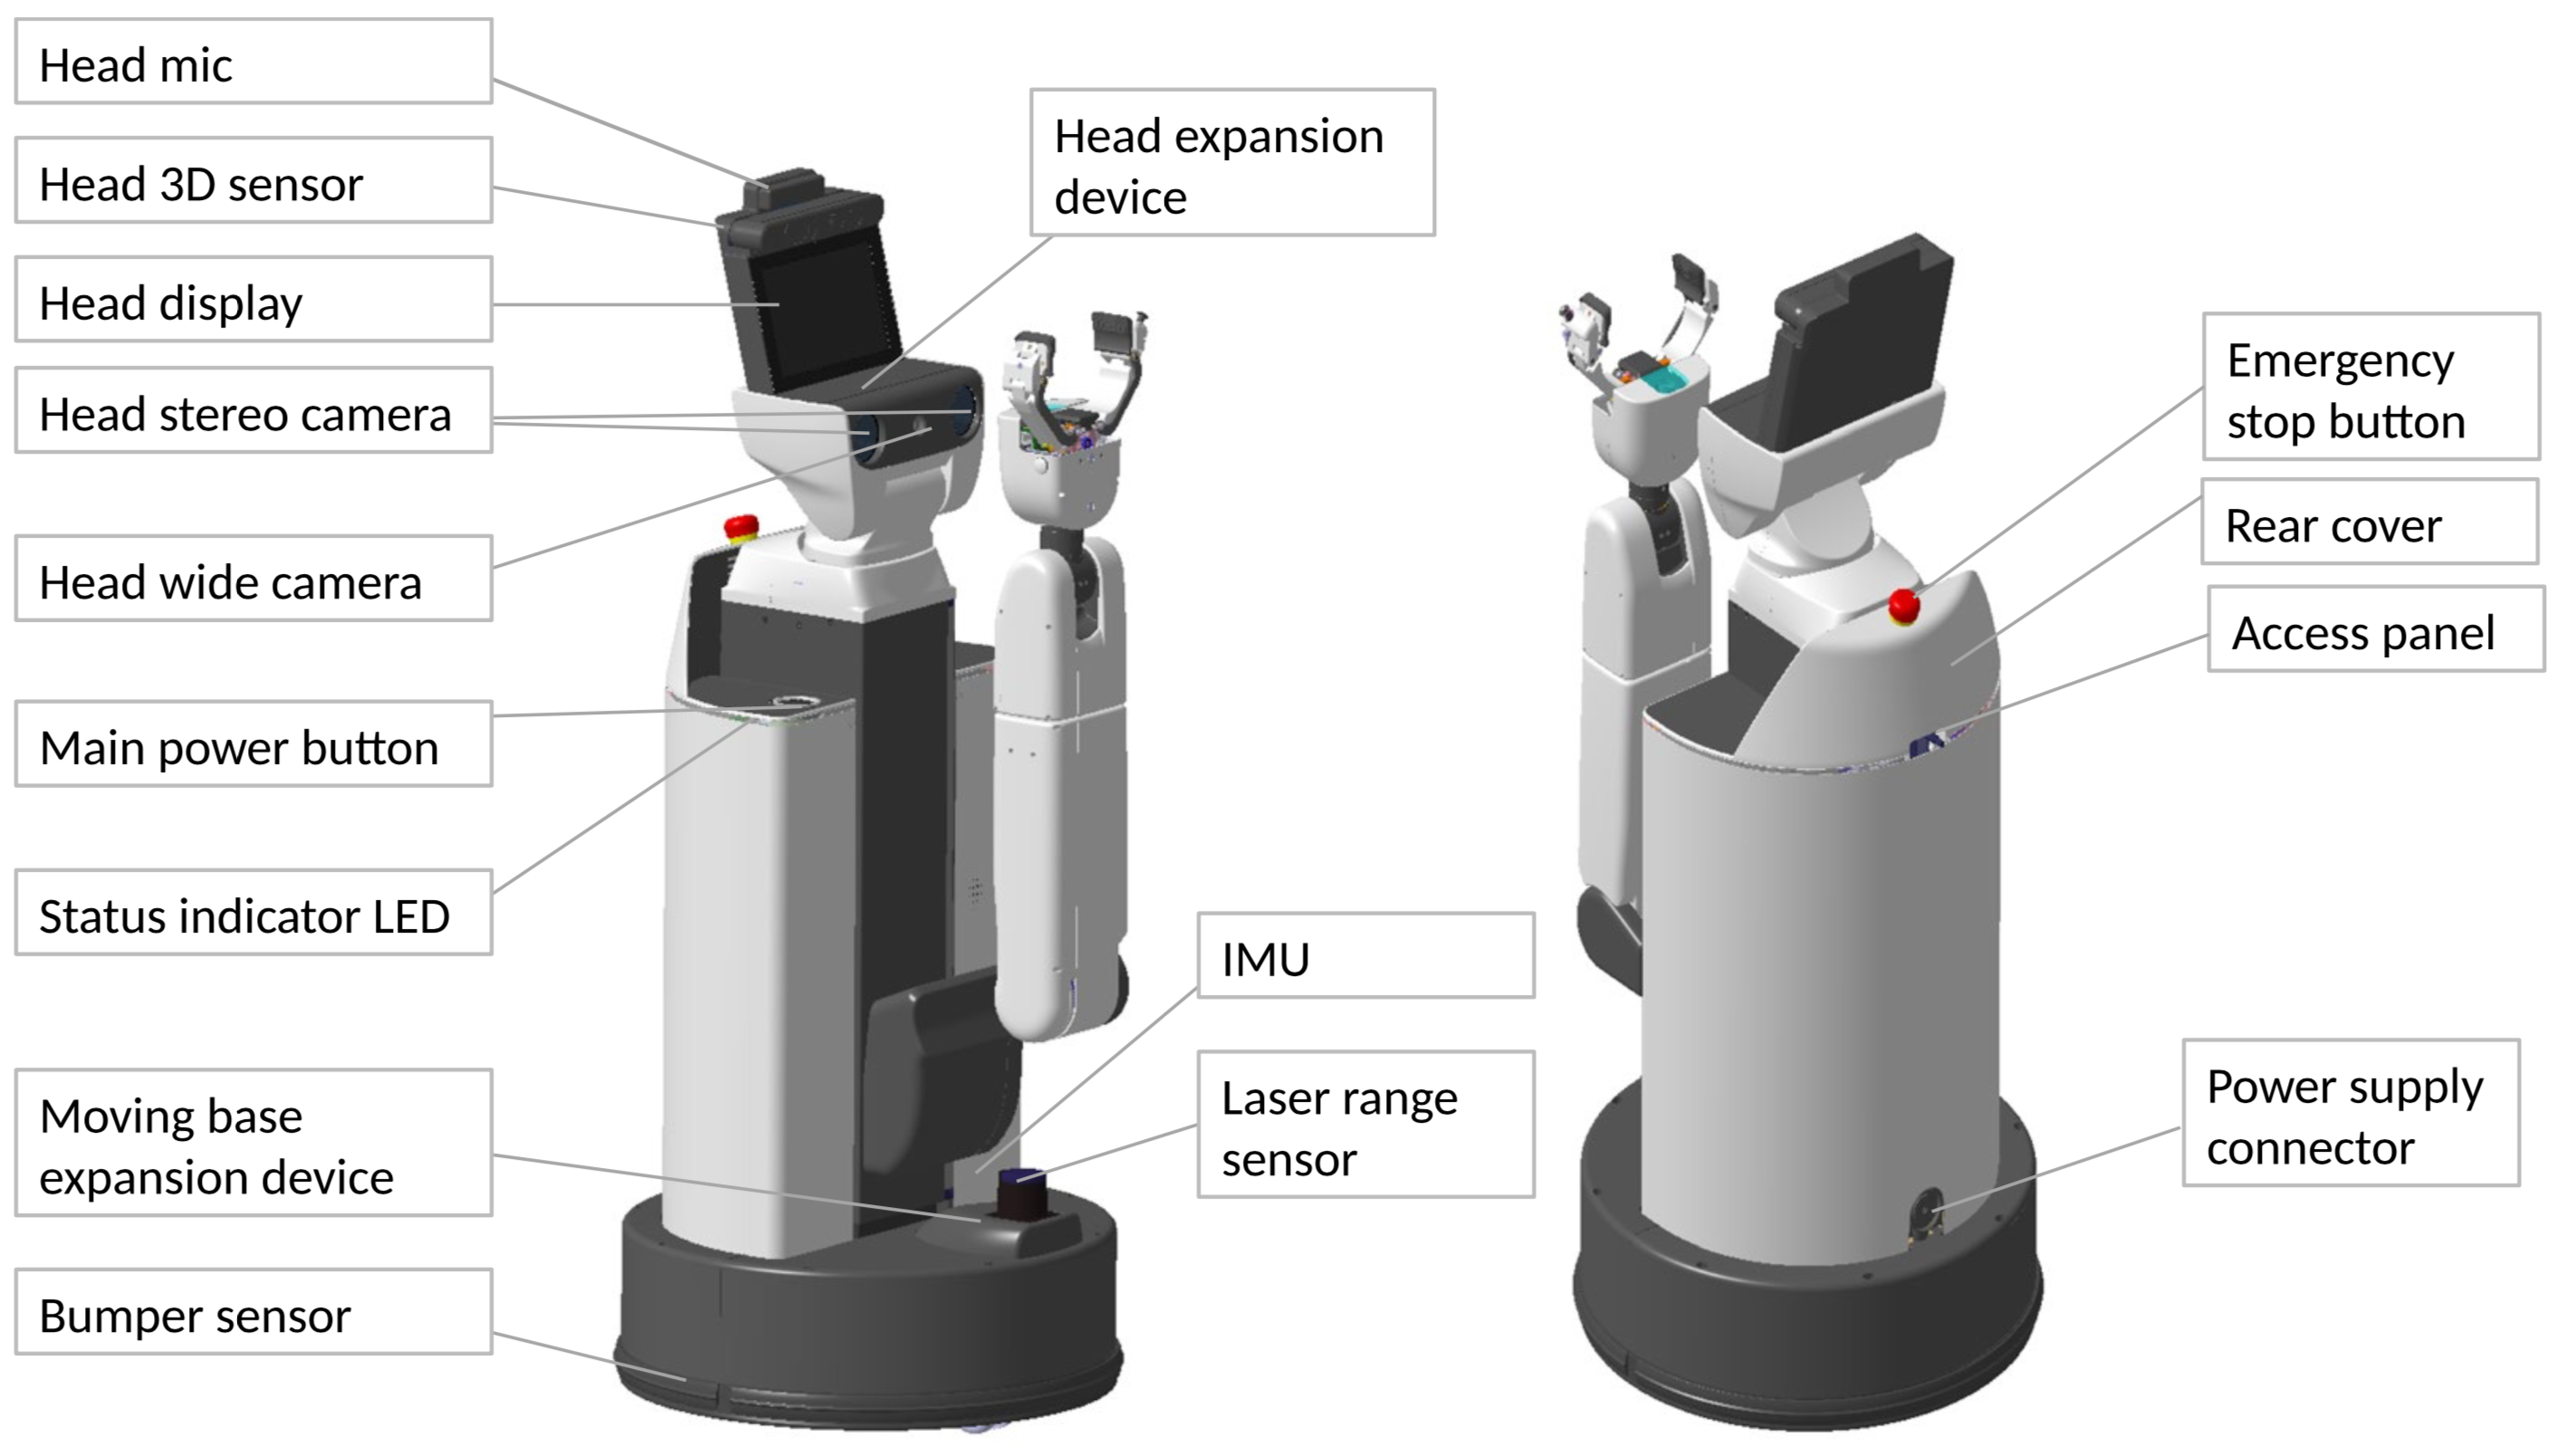
\includegraphics[width=\linewidth]{figure/chapter1/HSR_paper-2}
    \end{minipage}
    \begin{minipage}{0.39\hsize}
        \centering
        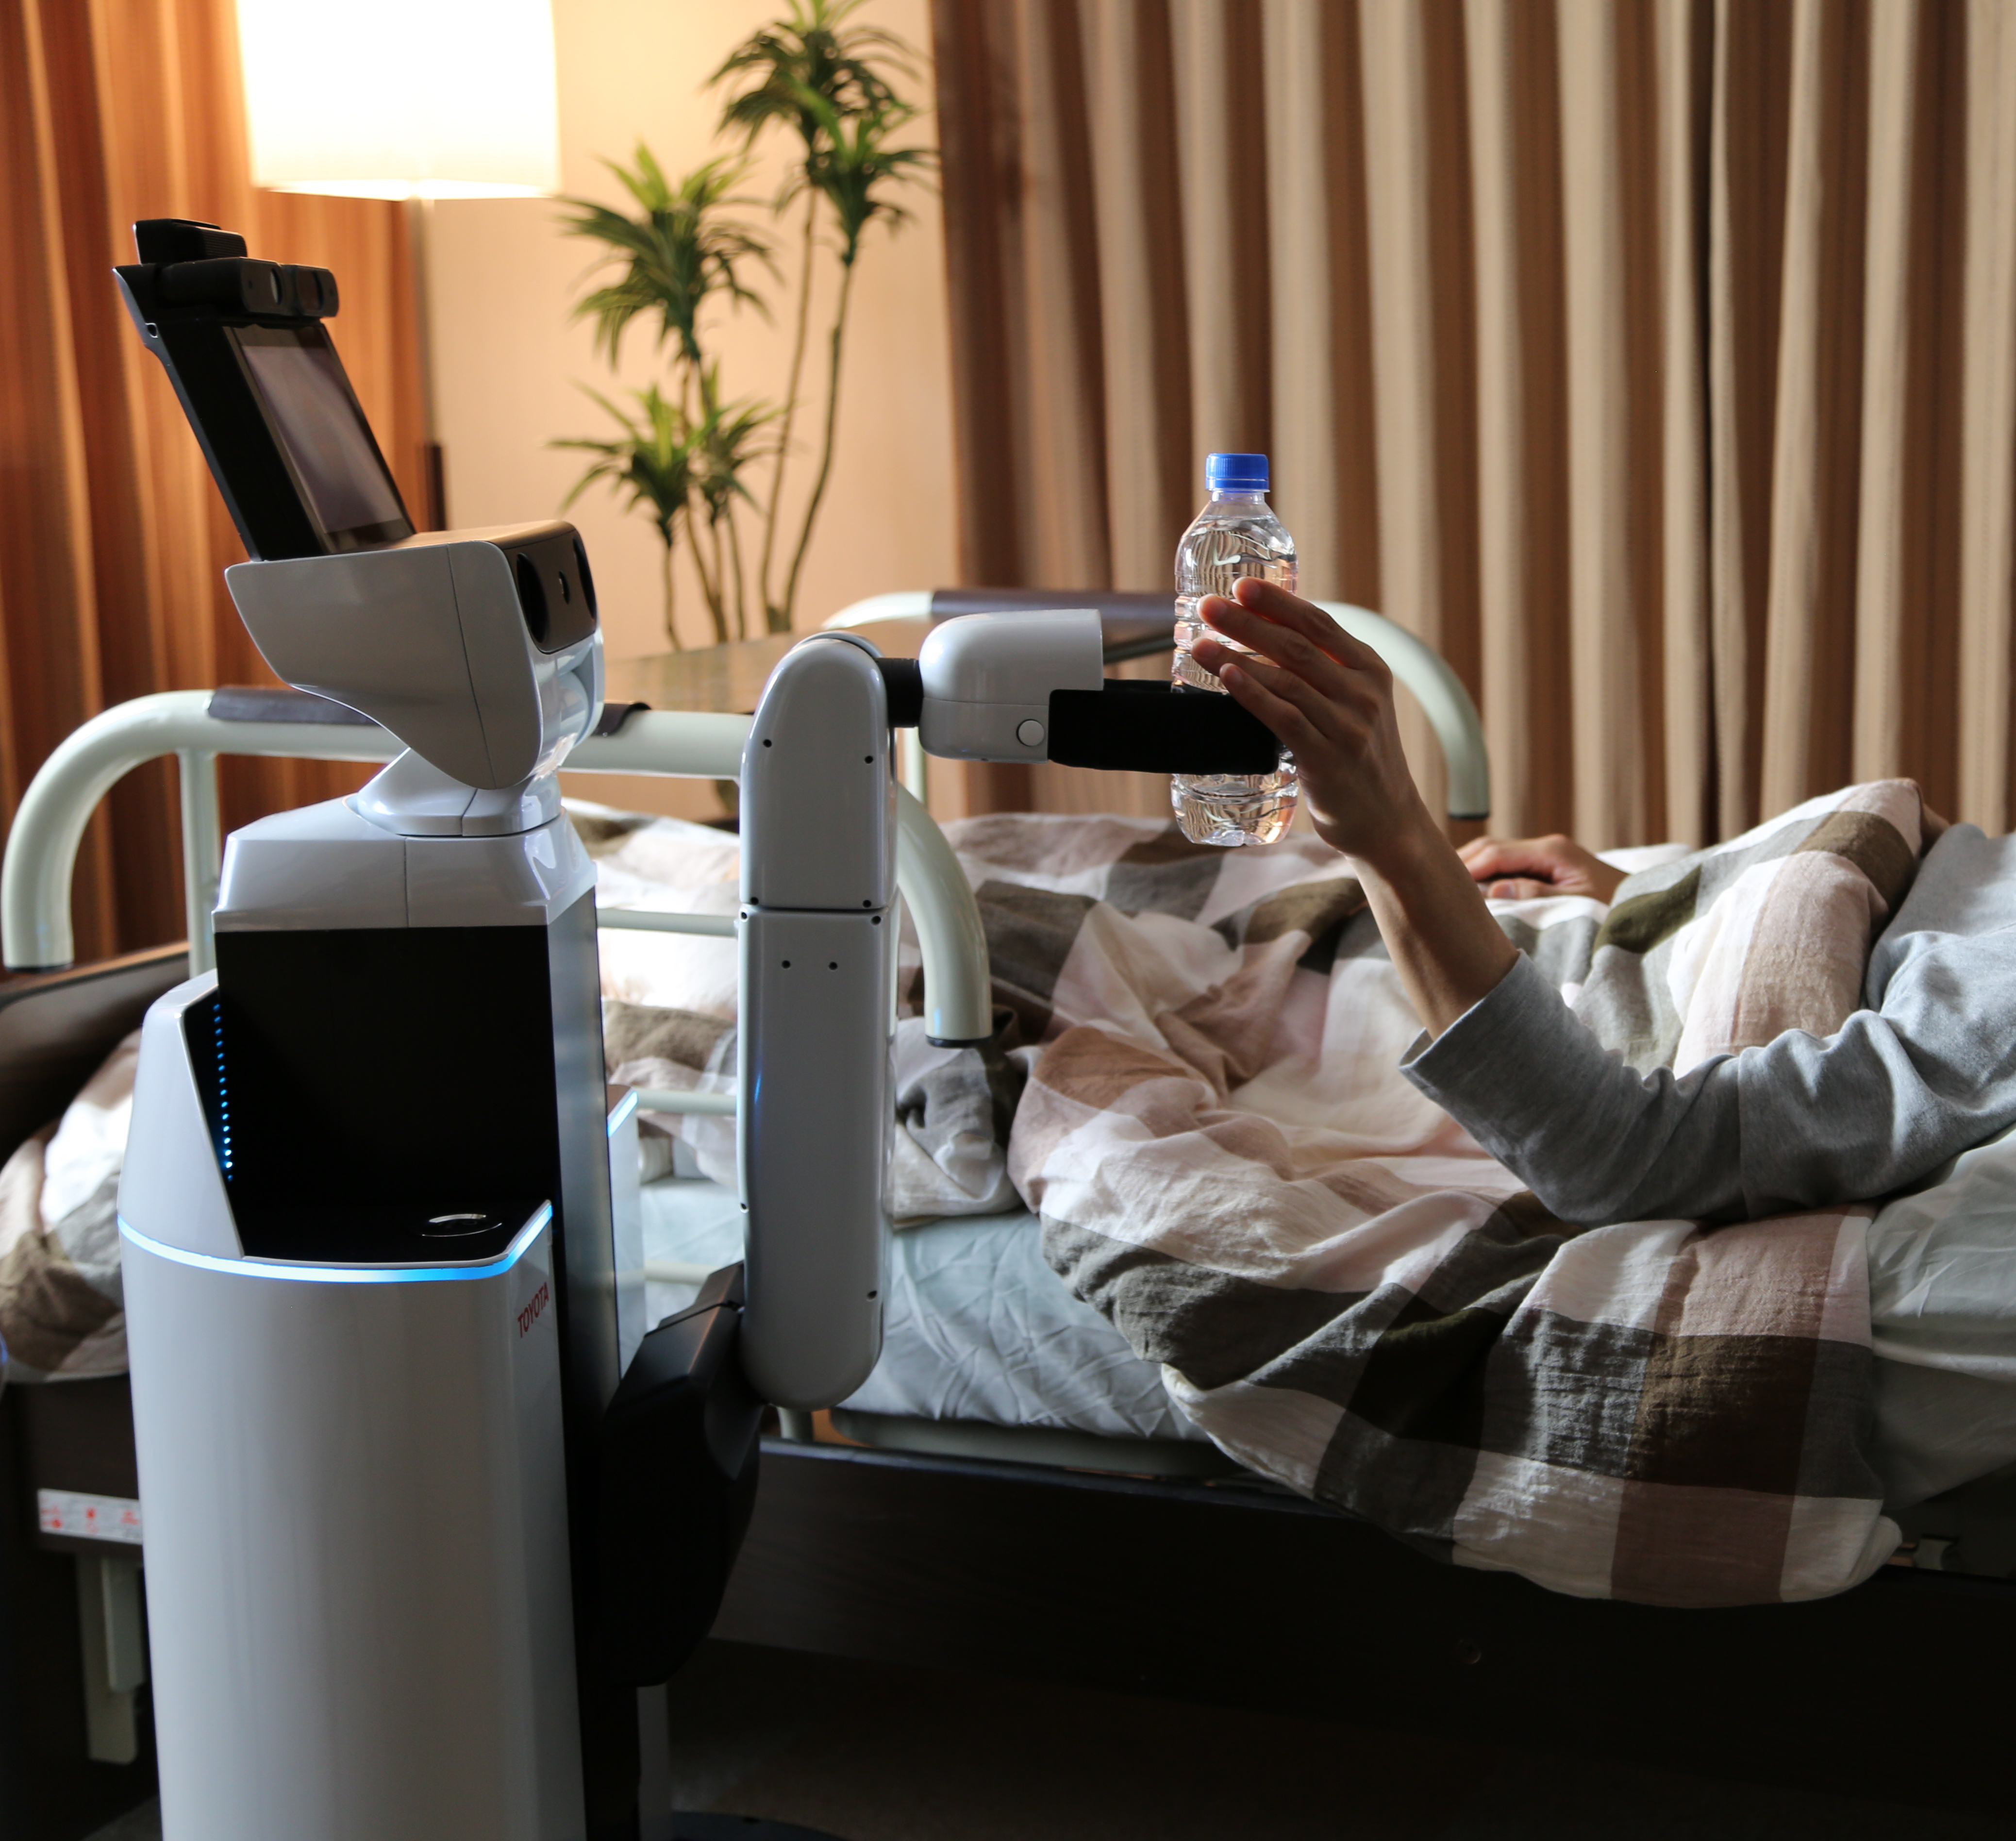
\includegraphics[width=\linewidth]{figure/chapter1/HSR_site-2}
    \end{minipage}
    \caption[Human Support Robot (HSR) produced by TOYOTA.]{Human Support Robot (HSR) produced by TOYOTA\cite{HSR2019, HSRサイト}.}
    \label{fig:HSR}
\end{figure}

筑波大の山海グループは片麻痺患者の日常生活を支援するサイバニックロボットアームを開発した\cite{Sankai2017, Sankai2019}.サイバニックアームは,片麻痺者の失われた上肢機能を代替可能なロボットアームとして,あたかも使用者の腕であるかのように人の意思に基づいて機能することを目標に開発された.ロボットアームは6自由度を持ち,非麻痺側の作業領域を狭めないようにテーブルタスクの領域をカバーする最小サイズで設計してある.グリッパに静電容量センサが搭載されており,これにより把持力と重心位置を把握できる.物体にかかる外力に基づいて健側腕の動きとその動作に関するユーザの意図を推定し,推定した情報に基づいて健側腕と協働して支援動作を提供することができる.ペットボトルやプリンの蓋など4種類の物体に対して開封の支援を検証した.音声入力に作業内容と対象物の認識を行い,ロボットアームで対象物を固定して,健常の腕でキャップなどの開封を行える.

サイバニックアームは机に固定して使用するため,持ち運びが困難であり自宅の特定の机でしか使用できない.また,事前に対象物の最適な把持力を教示させる必要がある.

\begin{figure}[H]
    \centering
    \begin{minipage}{0.49\hsize}
        \centering
        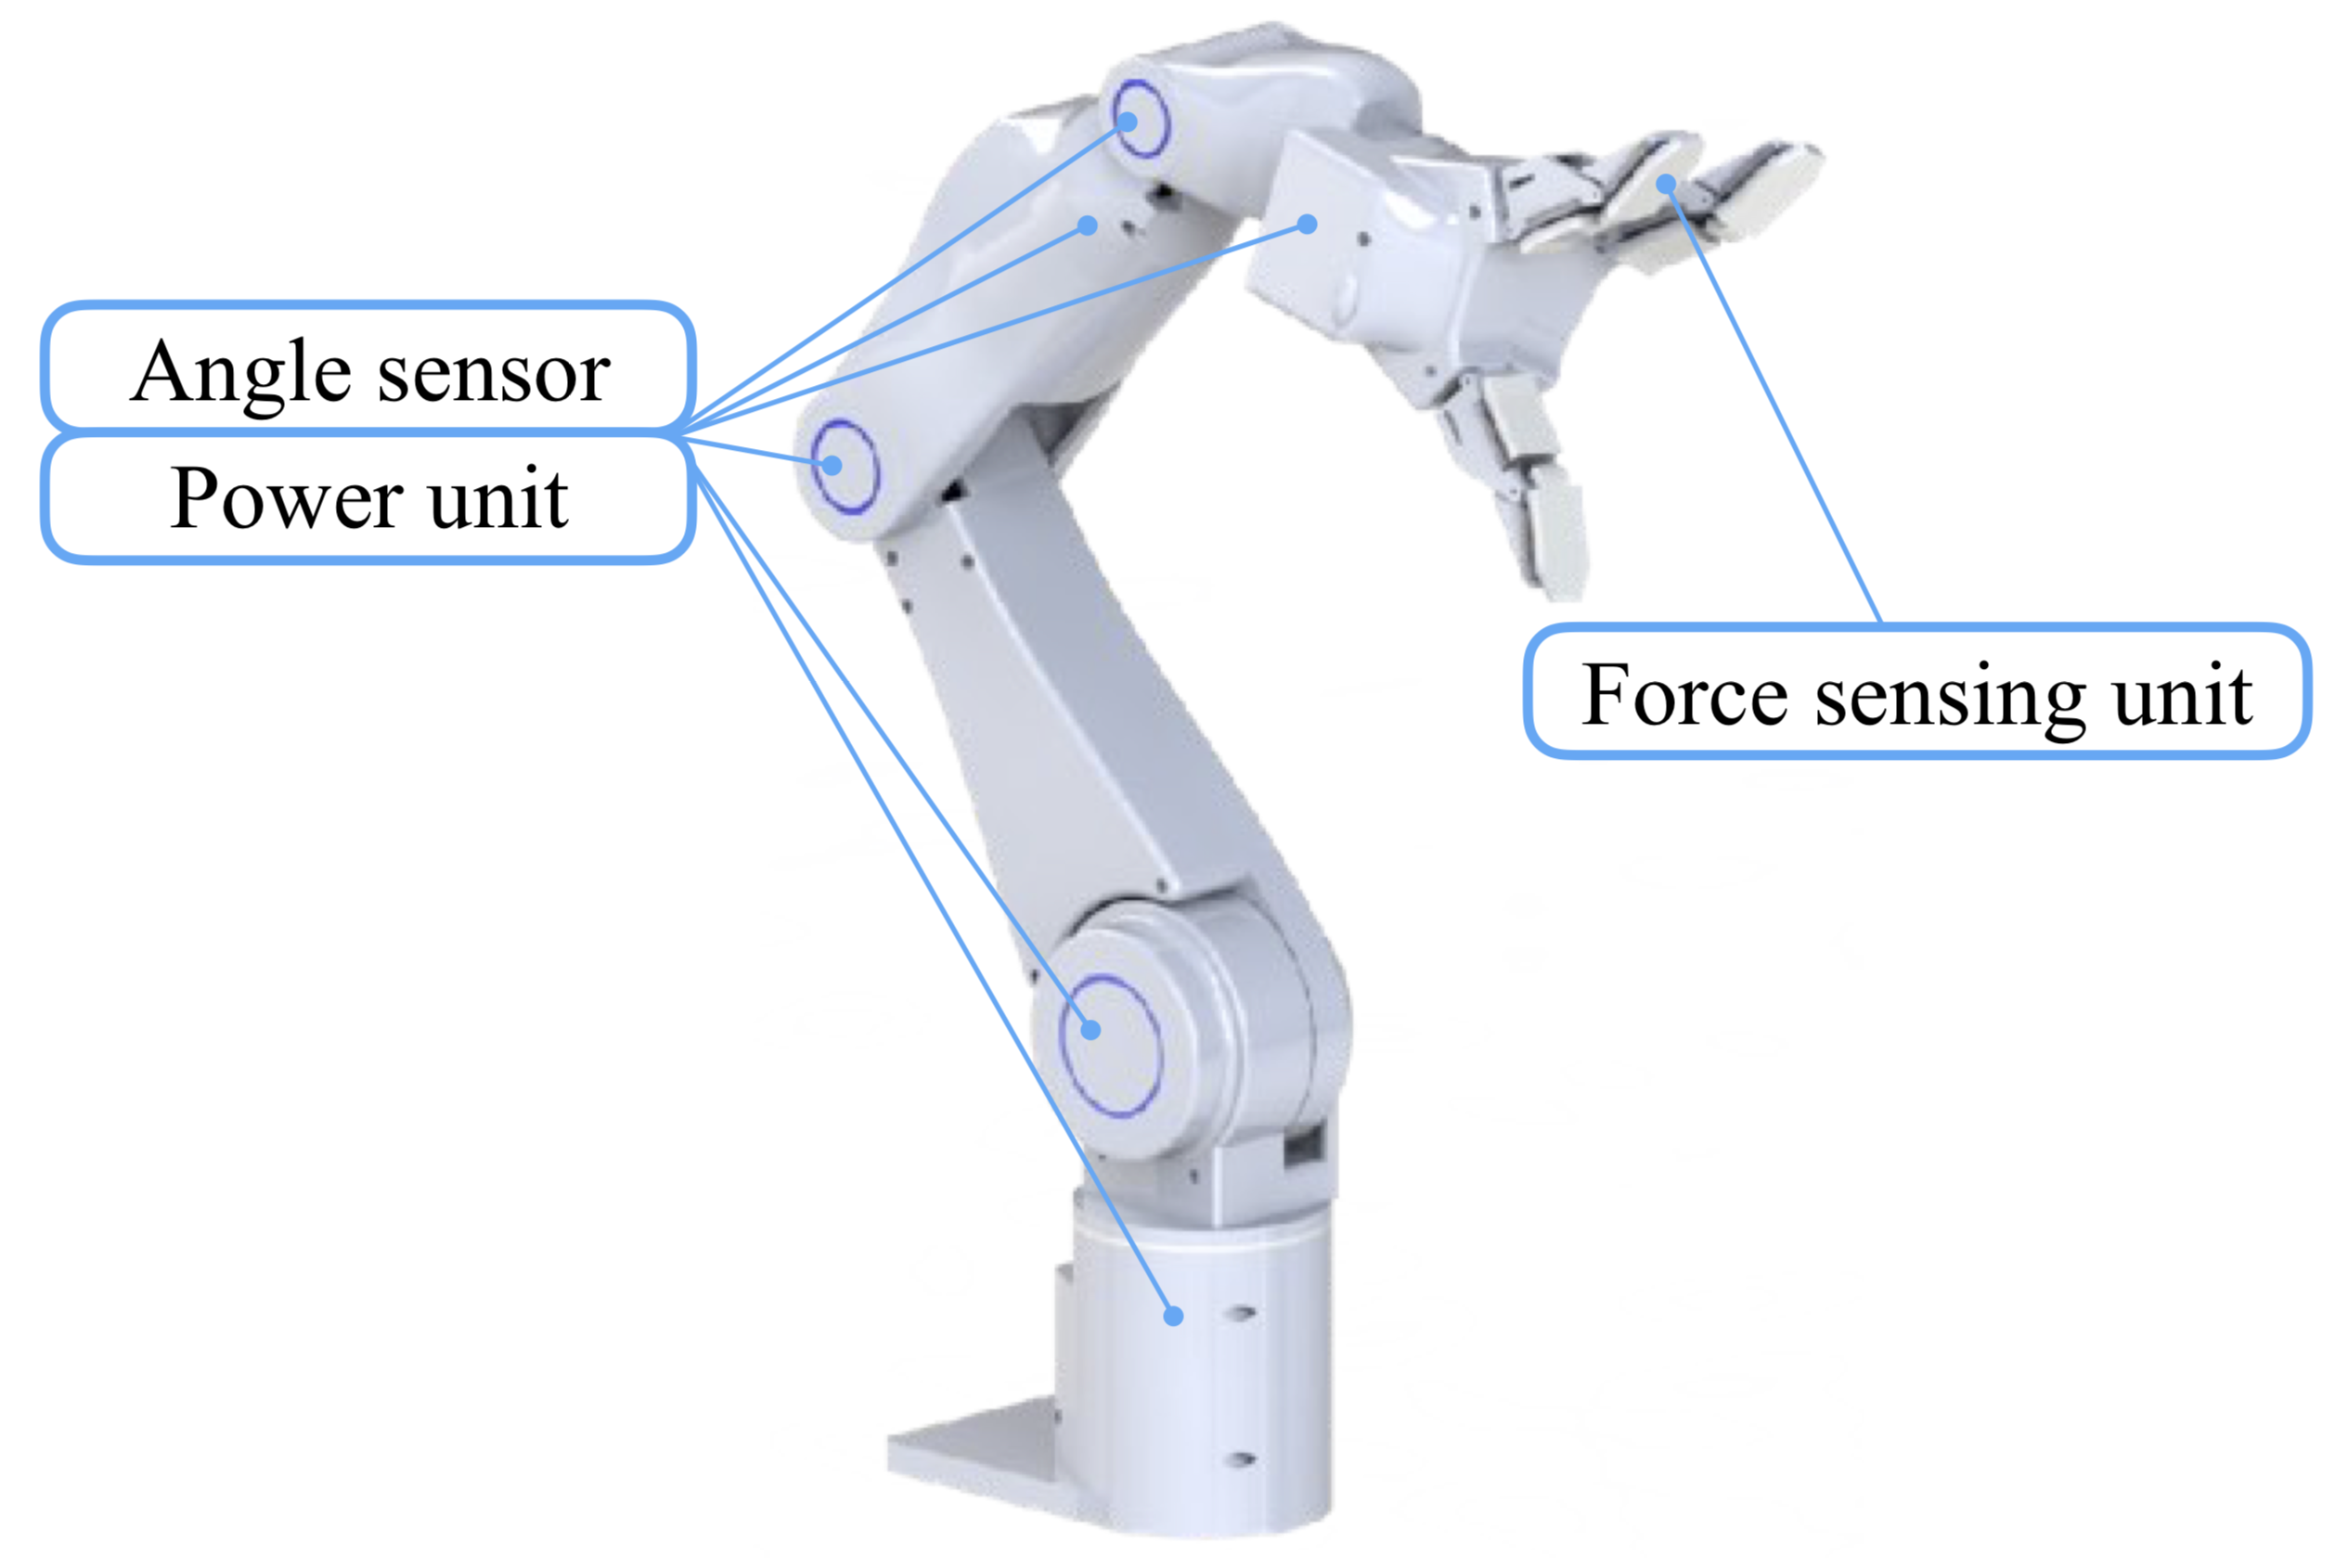
\includegraphics[width=\linewidth]{figure/chapter1/cybernic_arm_2017-2}
    \end{minipage}
    \begin{minipage}{0.49\hsize}
        \centering
        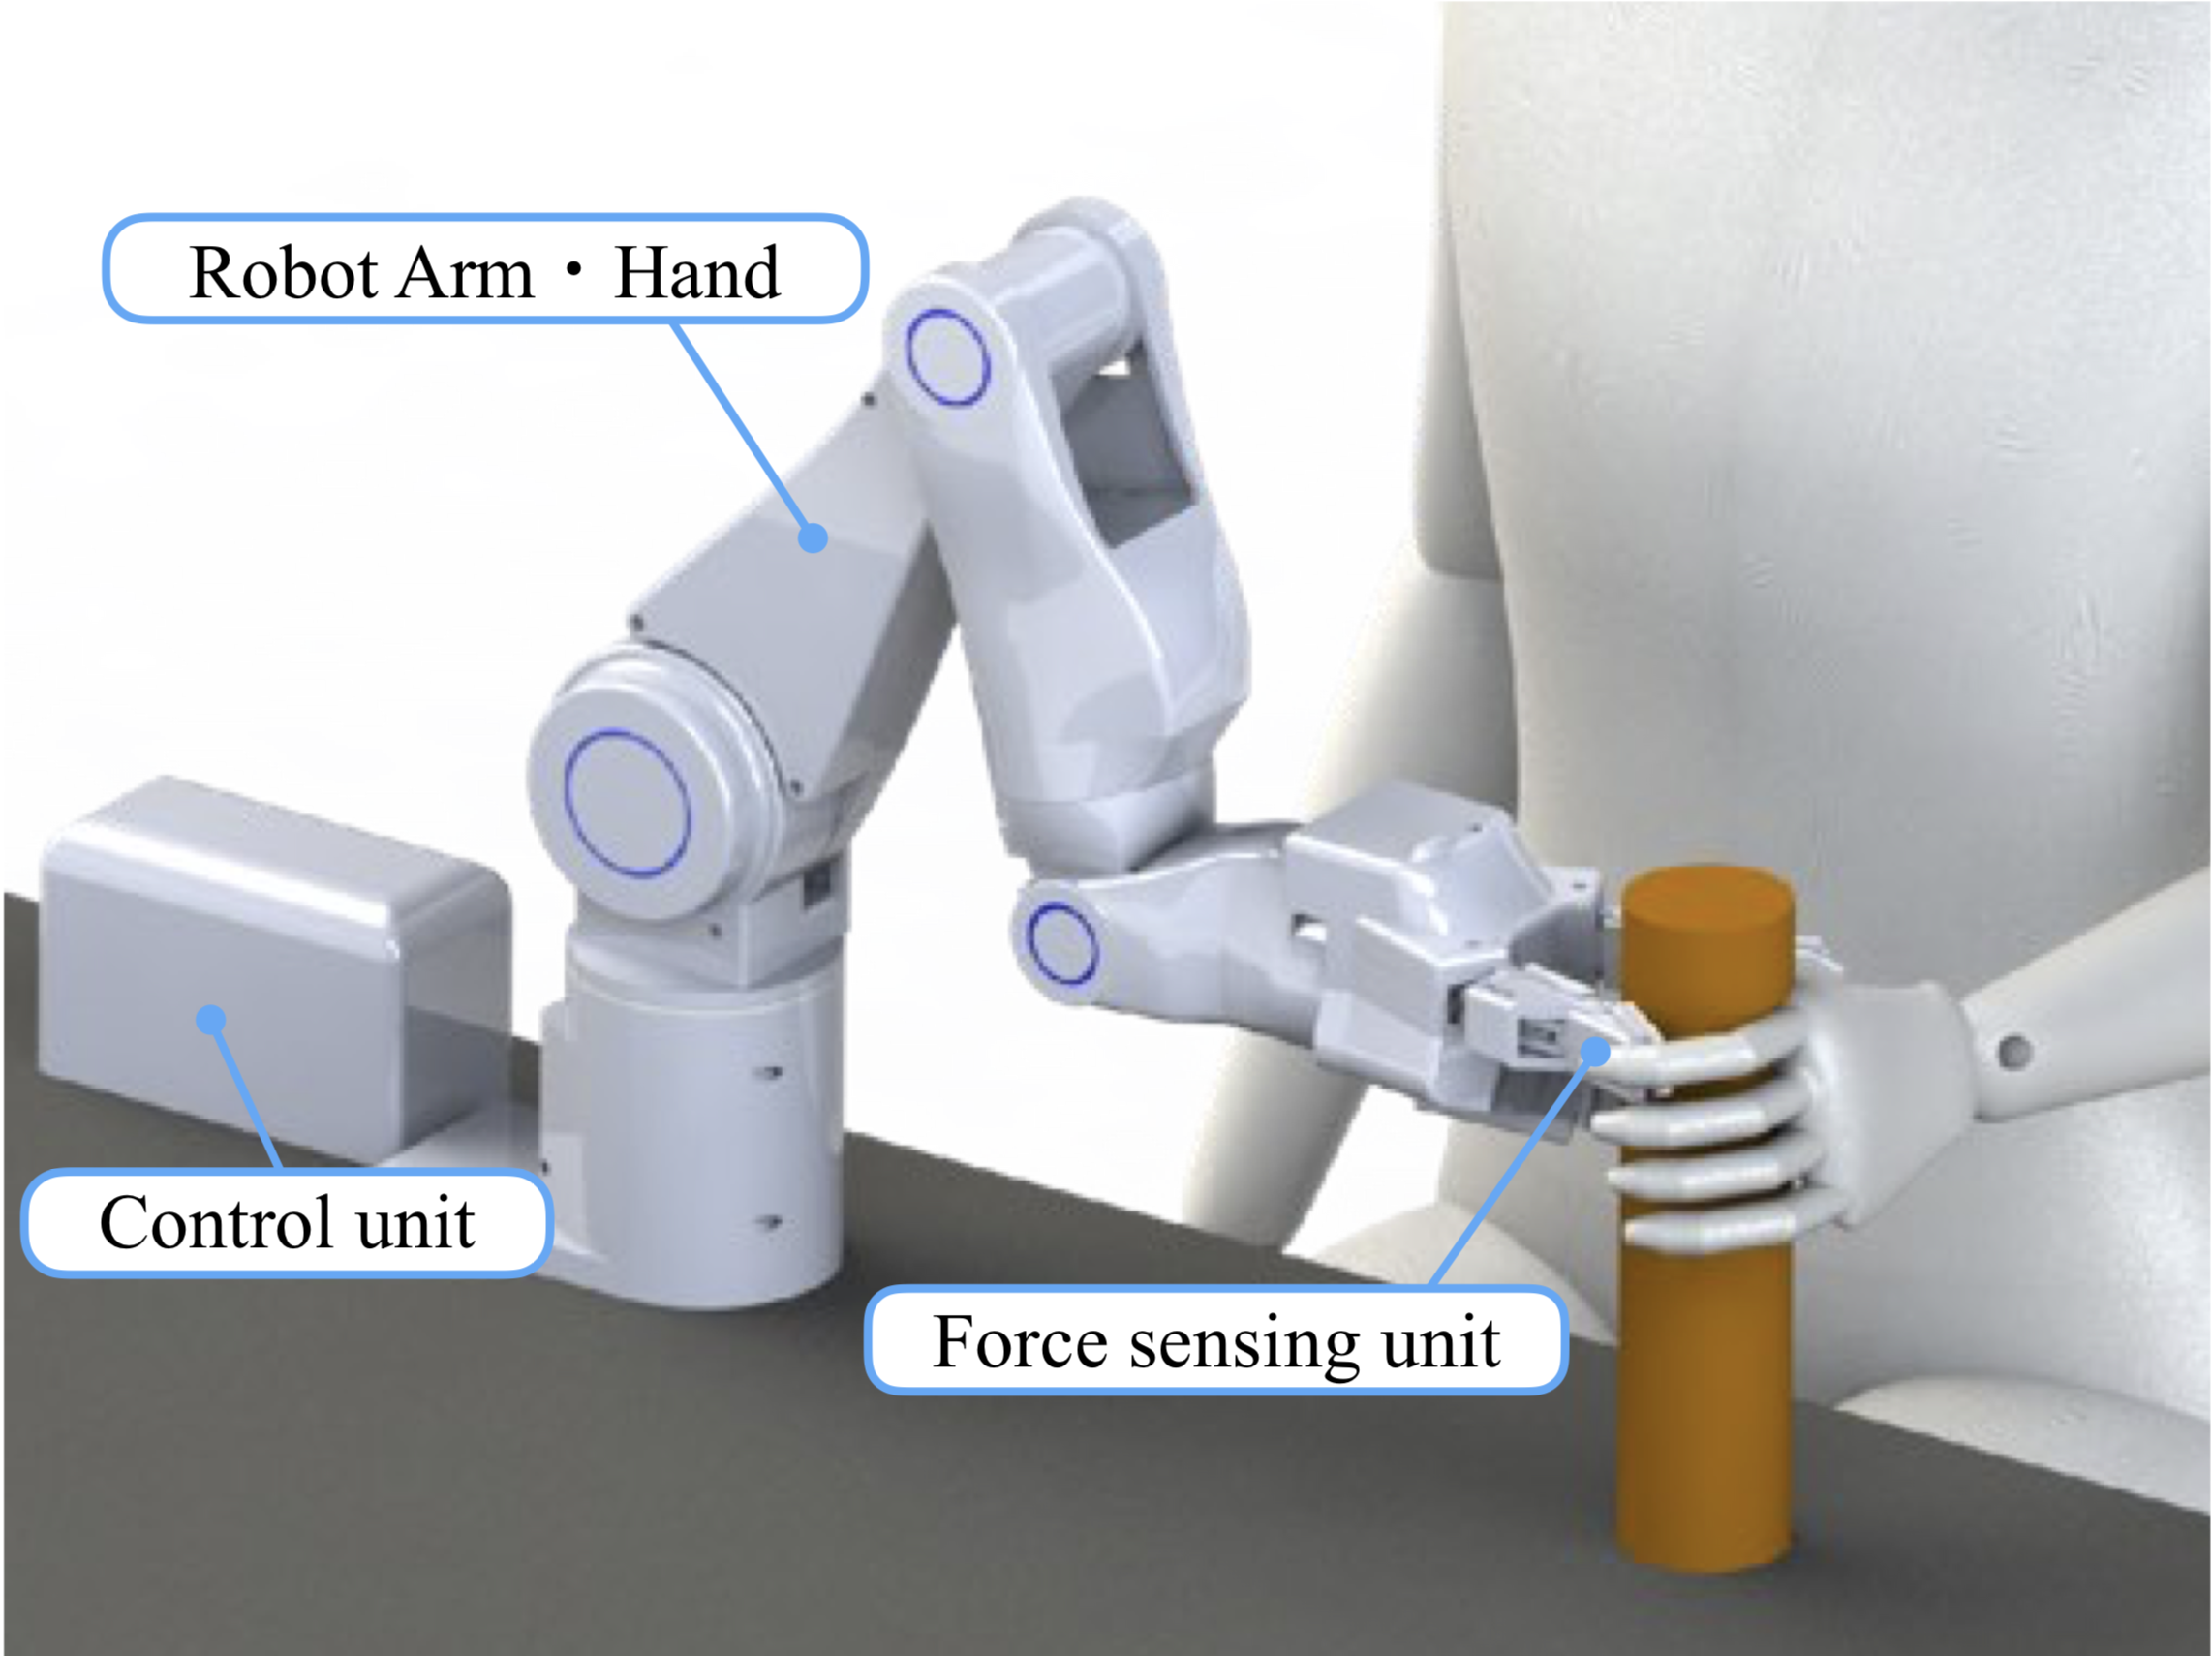
\includegraphics[width=\linewidth]{figure/chapter1/cybernic_arm_2017-1}
    \end{minipage}
    \begin{minipage}{\hsize}
        \centering
        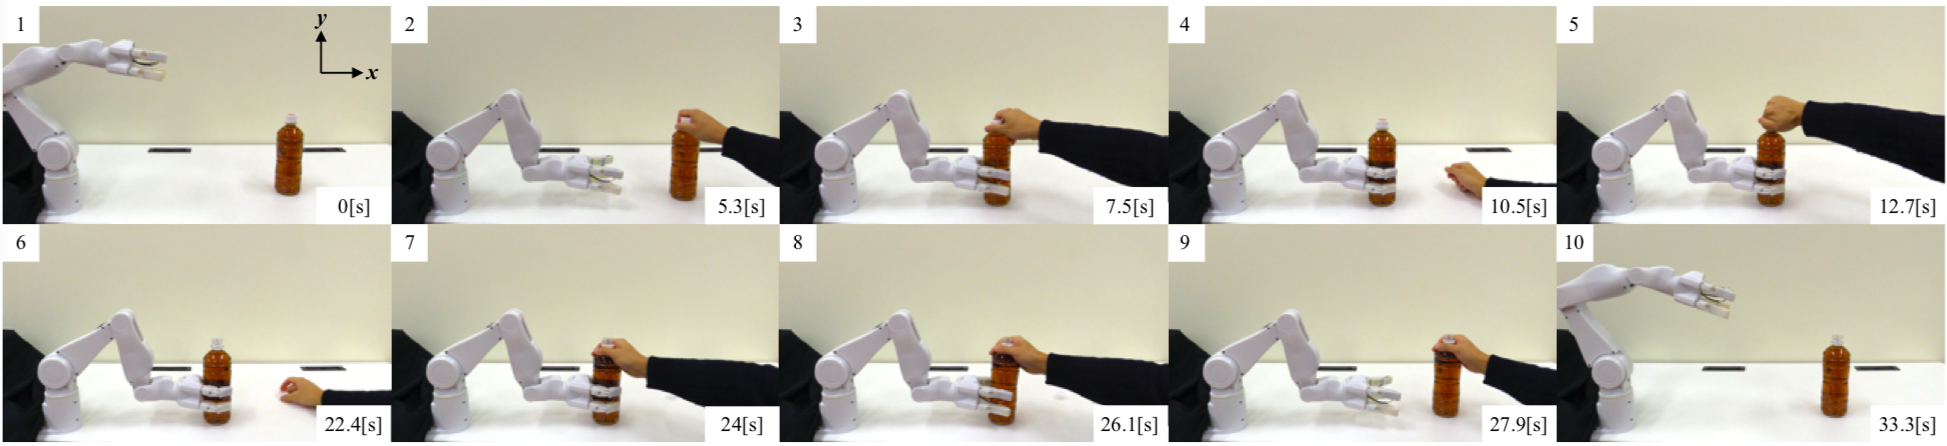
\includegraphics[width=\linewidth]{figure/chapter1/cybernic_arm_2019-3}
    \end{minipage}
    \caption[Cybernic robot arm produced by Sankai group.]{Cybernic robot arm produced by Sankai group\cite{Sankai2017, Sankai2019}.}
    \label{fig:cybernicarm}
\end{figure}


\section{研究目的}
% 筋電入力を避けた
% 自律走行するロボット
% ニーズを明確化する

本研究ではパーソナルロボットを小型化し,義手使用患者や片麻痺患者など上肢機能障害患者を対象としたパーソナルロボットを開発する.義手は常に身につけているように,パーソナルロボットも携帯できるよう小型化し腕の形をしたロボットハンドとする.制御の難しい筋電入力は避け,指令を与えると自律的に動作を行わせる.上肢機能障害者にとってはパーソナルロボットはどんな事態でも動作する必要があるため,今回はCloudは使用せずEdgeで処理を行うこととする.また座って机で作業することが多いため使用場所を机の上に限定し,指定した物をピックアップするパーソナルロボットハンドを作製することを目的とする.

\section{論文構成}
本論文は以下の章によって構成される.
\begin{enumerate}[\hspace{36pt}第1章\hspace{12pt}]
    \item 序論
    \item 深層学習とロボットへの応用
    \item 試作1号機の開発
    \item 試作2号機の開発
    \item 結論
\end{enumerate}
第1章では,ロボットの背景とその中でも医療・福祉ロボットの発展について述べ,研究目的を定めた.第2章では深層学習・強化学習の原理について述べ,深層学習を用いた画像認識技術および強化学習を用いたロボット制御について紹介する.第3章ではスマートフォンを搭載し,スマートフォンのCPUとカメラを用いたロボットハンド(1号機)の試作とその物理シミュレーションについて述べる.第4章では物体識別能力と把持機構を高性能化したロボットハンド(2号機)の試作について述べる.第5章では本論文を振り返り,1号機と2号機それぞれの達成点と課題点について述べ,次世代機の開発指針について言及し,今後の展望とする.

